\section{Solución de Schwarzschild}
\label{sec:solucionSchwarzschild}
\noindent La métrica de Schwarzschild fue la primera solución analítica a las ecuaciones de campo de Einstein. Esta solución comprende el caso mas sencillo posible, el de un objeto esféricamente simétrico y no rotante (Se puede ver la una traducción de la propuesta original en \cite{schwarzschild1999gravitationalfieldmasspoint}, en este texto haremos una derivación inspirada en \cite{eigenchris-2021}).
\begin{definition}{Condiciones de Schwarzschild}{}
    \begin{itemize}
        \item Tomamos un universo estático y esféricamente simétrico, es decir, un universo que no cambia con el tiempo y que tiene la misma forma en todas las direcciones.
        \item Se usan coordenadas esféricas $(t,r,\theta,\phi)$.
        \item Se Toma una masa puntual M en el origen de coordenadas.
        \item Se asume que no hay materia en el espacio-tiempo, es decir, que el tensor de energía-momento es cero.
        \item lejos de la masa puntual, el espacio-tiempo debe ser plano, es decir, la métrica debe ser la métrica de Minkowski.
    \end{itemize}
\end{definition}
Al saber que usaremos una simetría esférica, la métrica de Minkowski pasa de las componentes cartesianas a las componentes esféricas, es decir, la métrica de Minkowski en coordenadas esféricas es:
\begin{equation}
    \eta_{\mu \nu}=\left(\begin{array}{cccc}
            -1 & 0 & 0 & 0 \\
            0  & 1 & 0 & 0 \\
            0  & 0 & 1 & 0 \\
            0  & 0 & 0 & 1
        \end{array}\right)=\left(\begin{array}{cccc}
            -1 & 0 & 0     & 0                      \\
            0  & 1 & 0     & 0                      \\
            0  & 0 & r^{2} & 0                      \\
            0  & 0 & 0     & r^{2} \sin ^{2} \theta
        \end{array}\right)
\end{equation}
y
\begin{equation}
    \eta^{\mu \nu}=\left(\begin{array}{cccc}
            -1 & 0 & 0 & 0 \\
            0  & 1 & 0 & 0 \\
            0  & 0 & 1 & 0 \\
            0  & 0 & 0 & 1
        \end{array}\right)=\left(\begin{array}{cccc}
            -1 & 0 & 0               & 0                                \\
            0  & 1 & 0               & 0                                \\
            0  & 0 & \frac{1}{r^{2}} & 0                                \\
            0  & 0 & 0               & \frac{1}{r^{2} \sin ^{2} \theta}
        \end{array}\right),
\end{equation}
se considera que cuando la variable $r$ tiende a infinito la métrica se acerca asintóticamente a Minkowski. A continuación escribiremos que implicaciones tiene cada condición.

\subsubsection*{Estático en el tiempo}

La métrica de Schwarzschild describe el espacio-tiempo exterior a una distribución esféricamente simétrica de masa en vacío. Una de sus propiedades fundamentales es que es \textbf{estática}, lo que significa que el espacio-tiempo no cambia con el tiempo y no presenta términos de arrastre (frame-dragging).

Formalmente, una solución es estática si cumple dos condiciones:
1. Es \textbf{estacionaria}, es decir, existe un vector de Killing temporal que refleja la invariancia bajo traslaciones en el tiempo.
2. Es \textbf{irrotacional}, lo que implica que el vector de Killing temporal es ortogonal a las hipersuperficies espaciales.

\begin{definition}{Implicaciones para una solución estática}{}
    \begin{itemize}
        \item Existe un vector de Killing temporal \( \xi^\mu \) tal que \( \nabla_{(\mu} \xi_{\nu)} = 0 \).
        \item La métrica no depende explícitamente de la coordenada temporal:
              \[ \partial_t g_{\mu \nu} = 0. \]
        \item La reversión temporal \( t \to -t \) deja invariante la métrica:
              \[ g_{\mu\nu}(t) = g_{\mu\nu}(-t). \]
        \item No hay términos cruzados entre las coordenadas espaciales y temporales, es decir:
              \[ g_{ti} = 0, \quad \forall i \in \{r, \theta, \phi\}. \]
    \end{itemize}
\end{definition}

A partir de esta propiedad, la métrica en coordenadas de tipo \((t, r, \theta, \phi)\) adopta la forma general:

\begin{equation}
    g_{\mu \nu} =
    \begin{bmatrix}
        g_{tt} & 0            & 0                & 0              \\
        0      & g_{rr}       & g_{r\theta}      & g_{r\phi}      \\
        0      & g_{\theta r} & g_{\theta\theta} & g_{\theta\phi} \\
        0      & g_{\phi r}   & g_{\phi\theta}   & g_{\phi\phi}
    \end{bmatrix}.
\end{equation}

Debido a la simetría esférica de Schwarzschild, los términos fuera de la diagonal desaparecen, quedando únicamente las componentes \( g_{tt} \) y \( g_{rr} \) como funciones de \( r \). En secciones posteriores, exploraremos cómo esta estructura nos lleva a la forma explícita de la métrica de Schwarzschild.


\subsubsection*{Simetría esférica}
Debido a que estamos usando una simetría esférica se debe cumplir:
\begin{itemize}
    \item Los componentes $\theta, \phi$ deben usar la métrica para una esfera de radio $r$.
    \item Permitir una función de escala radial $C(r)$.
\end{itemize}

\begin{equation}
    \begin{array}{ll}
        g_{\theta \theta} & g_{\theta \phi} \\
        g_{\phi \theta}   & g_{\phi \phi}
    \end{array} = \left[\begin{array}{cc}
            C(r) r^2 & 0                       \\
            0        & C(r) r^2(\sin \theta)^2
        \end{array}\right].
\end{equation}
Ahora para los demás componentes de la métrica considerando a la ortogonalidad de los vectores base
\begin{equation}
    \begin{aligned}
         & \overrightarrow{e_\theta} \cdot \overrightarrow{e_r}=0=g_{\theta r} \\
         & \overrightarrow{e_\phi} \cdot \overrightarrow{e_r}=0=g_{\phi r},
    \end{aligned}
\end{equation}
es posible escribir la métrica de forma diagonal
\begin{equation}
    \left[\begin{array}{cccc}
            g_{t t}(r, \theta, \phi) & 0                        & 0        & 0                       \\
            0                        & g_{r r}(r, \theta, \phi) & 0        & 0                       \\
            0                        & 0                        & C(r) r^2 & 0                       \\
            0                        & 0                        & 0        & C(r) r^2(\sin \theta)^2
        \end{array}\right].
\end{equation}
Una noción clave para facilitar los cálculos es que estamos tomando en consideración una masa puntual en un universo vacío e isotrópico, así que es de esperarse que la métrica no dependa de las coordenadas $\theta$ y $\phi$, permitiéndonos escribirla solo en términos de la distancia al origen $r$ tal que
\begin{equation}
    \left[\begin{array}{cccc}
            -A(r) & 0    & 0        & 0                       \\
            0     & B(r) & 0        & 0                       \\
            0     & 0    & C(r) r^2 & 0                       \\
            0     & 0    & 0        & C(r) r^2(\sin \theta)^2
        \end{array}\right].
\end{equation}
A continuación se tomará el siguiente cambio de variable:

\begin{equation}
    \tilde{r}=\sqrt{C(r)} \, r
\end{equation}
La forma de proceder va a ser  que cuando estemos lejos de la masa $M$, debemos tener las ecuaciones de campo débil a bajas velocidades y recuperar las ecuaciones de Newton.
\begin{equation*}
    g_{\mu \nu} \rightarrow \Gamma_{\mu \nu}^\sigma \rightarrow R_{\mu \nu} \rightarrow \text{Gravedad Newtoniana}
\end{equation*}


\subsubsection{Christoffel symbols}
los símbolos de Christoffel
\begin{equation}
    \begin{gathered}
        \Gamma_{\mu \nu}^0 \rightarrow\left[\begin{array}{cccc}
                0                        & \frac{\partial_r A}{2 A} & 0 & 0 \\
                \frac{\partial_r A}{2 A} & 0                        & 0 & 0 \\
                0                        & 0                        & 0 & 0 \\
                0                        & 0                        & 0 & 0
            \end{array}\right]
        \quad
        \Gamma_{\mu \nu}^1 \rightarrow\left[\begin{array}{cccc}
                \frac{\partial_r A}{2 B} & 0                        & 0            & 0                           \\
                0                        & \frac{\partial_r B}{2 B} & 0            & 0                           \\
                0                        & 0                        & -\frac{r}{B} & 0                           \\
                0                        & 0                        & 0            & -\frac{r(\sin \theta)^2}{B}
            \end{array}\right] \\
        \Gamma_{\mu \nu}^2 \rightarrow\left[\begin{array}{cccc}
                0 & 0           & 0           & 0                        \\
                0 & 0           & \frac{1}{r} & 0                        \\
                0 & \frac{1}{r} & 0           & 0                        \\
                0 & 0           & 0           & -\sin \theta \cos \theta
            \end{array}\right]
        \quad
        \Gamma_{\mu \nu}^3 \rightarrow\left[\begin{array}{cccc}
                0 & 0           & 0           & 0           \\
                0 & 0           & 0           & \frac{1}{r} \\
                0 & 0           & 0           & \cot \theta \\
                0 & \frac{1}{r} & \cot \theta & 0
            \end{array}\right]
    \end{gathered}
\end{equation}

\begin{equation}
    \begin{gathered}
        \Gamma_{01}^0=\Gamma_{10}^0=\frac{1}{2} \frac{1}{A}\left(\partial_r A\right), \quad \Gamma_{00}^1=\frac{1}{2} \frac{1}{B}\left(\partial_r A\right) \\
        \Gamma_{11}^1=\frac{11}{2} \frac{1}{B}\left(\partial_r B\right), \quad \Gamma_{22}^1=-\frac{r}{B}, \quad \Gamma_{33}^1=-\frac{r(\sin \theta)^2}{B} \\
        \Gamma_{12}^2=\Gamma_{21}^2=\Gamma_{13}^3=\Gamma_{31}^3=\frac{1}{r}, \quad \Gamma_{33}^2=-\sin \theta \cos \theta, \quad \Gamma_{23}^3=\Gamma_{32}^3=\cot \theta
    \end{gathered}
\end{equation}

Calculate:
- $R_{00}=0$
- $R_{11}=0$
$R_{\mu \nu}=0$
- $R_{22}=0$

\begin{equation}
    R_{00}=\frac{\partial_r \partial_r A}{2 B}
    -\frac{\partial_r A \,\partial_r B}{4 B^2}
    +\frac{\partial_r A}{B r}
    -\frac{\left(\partial_r A\right)^2}{4 A B}=0
\end{equation}

\begin{equation}
    R_{00}+R_{11}=0
\end{equation}

\begin{equation}
    \begin{aligned}
        g_{\mu \nu} & \rightarrow\left[\begin{array}{cccc}
                                               A(r) & 0     & 0    & 0                   \\
                                               0    & -B(r) & 0    & 0                   \\
                                               0    & 0     & -r^2 & 0                   \\
                                               0    & 0     & 0    & -r^2(\sin \theta)^2
                                           \end{array}\right] \\
        g_{\mu \nu} & \rightarrow\left[\begin{array}{cccc}
                                               1 & 0  & 0    & 0                   \\
                                               0 & -1 & 0    & 0                   \\
                                               0 & 0  & -r^2 & 0                   \\
                                               0 & 0  & 0    & -r^2(\sin \theta)^2
                                           \end{array}\right]
    \end{aligned}
\end{equation}

\begin{equation}
    \begin{gathered}
        B A^{\prime}+A B^{\prime}=0 \\
        \partial_r(A B)=0 \\
        \Rightarrow A B=K
    \end{gathered}
\end{equation}
\begin{equation}
    \begin{aligned}
         & A(r) \rightarrow 1 \\
         & B(r) \rightarrow 1
    \end{aligned}
\end{equation}
\begin{equation}
    (1)(1)=K
\end{equation}

\begin{equation}
    \Rightarrow B(r)=\frac{1}{A(r)} \text { para todo } r
\end{equation}

\begin{equation}
    B^{\prime}=\partial_r\left(A^{-1}\right)=-\frac{A^{\prime}}{A^2}
\end{equation}


\begin{equation}
    \begin{aligned}
         & R_{22}=-2 A B+2 A B^2-r A^{\prime} B+r A B^{\prime}                                                               \\
         & 0=-2 A \frac{1}{A}+2 A\left(\frac{1}{A}\right)^2-r A^{\prime} \frac{1}{A}+r A\left(-\frac{A^{\prime}}{A^2}\right)
    \end{aligned}
\end{equation}
\begin{equation}
    \Rightarrow r A^{\prime}=1-A
\end{equation}

\begin{equation}
    \begin{aligned}
         & \frac{A(r)}{\partial} \equiv 1-\frac{k^{\prime}}{r}                                 \\
         & \frac{\partial}{\partial r} A=\frac{\partial}{\partial r}\left(1-\frac{k}{r}\right) \\
         & A^{\prime}=\frac{\partial}{\partial r} 1-k \frac{\partial}{\partial r} r^{-1}       \\
         & A^{\prime}=0                                                                        \\
         & A^{\prime}=\frac{k}{r^2}
    \end{aligned}
\end{equation}

\begin{equation}
    g_{\mu \nu} \rightarrow\left[\begin{array}{cccc}
            1-\frac{k}{r} & 0                                & 0    & 0                   \\
            0             & -\left(1-\frac{k}{r}\right)^{-1} & 0    & 0                   \\
            0             & 0                                & -r^2 & 0                   \\
            0             & 0                                & 0    & -r^2(\sin \theta)^2
        \end{array}\right]
\end{equation}

\begin{task}{}{}
    Terminar la derivación
\end{task}
La métrica de Schwarzschild es:
\begin{equation}
    \boxed{g_{\mu \nu}=\left(\begin{array}{cccc}
                -1+\frac{2 G m}{r c^2} & 0                                       & 0   & 0                  \\
                0                      & \left(1-\frac{2 G m}{r c^2}\right)^{-1} & 0   & 0                  \\
                0                      & 0                                       & r^2 & 0                  \\
                0                      & 0                                       & 0   & r^2 \sin ^2 \theta
            \end{array}\right)}
\end{equation}
\subsection{Geodésicas en Schwarzschild tipo  nulas}

El movimiento de los cuerpos y de la luz en el espacio-tiempo de Schwarzschild está dado por la ecuación geodésica:
\begin{equation}
    \frac{\mathrm{d}^2 x^\mu}{\mathrm{d} \lambda^2}+\Gamma^\mu{ }_{\nu \rho} \frac{\mathrm{~d} x^\nu}{\mathrm{d} \lambda} \frac{\mathrm{~d} x^\rho}{\mathrm{d} \lambda}=0
    \label{eq:geodesic}
\end{equation}
Con $X^0 = ct$, $X^1 = r$, $X^2 = \theta$, $X^3 = \phi$ y $\lambda$ es un parámetro afín.

Donde los símbolos de Christoffel no cero son:
$$
    \begin{array}{l}
        \Gamma^0{ }_{10}=\Gamma^0{ }_{01}=\dfrac{G M}{c^2 r\left(r - \dfrac{2 G M}{c^2}\right)},                                                                                                                       \\
        \Gamma^1{ }_{11}=-\dfrac{G M}{c^2 r\left(r - \dfrac{2 G M}{c^2}\right)}, \quad \Gamma^1{ }_{22}=-\left(r - \dfrac{2 G M}{c^2}\right), \quad \Gamma^1{ }_{33}=-\left(r - \dfrac{2 G M}{c^2}\right) \sin \theta, \\
        \Gamma^2{ }_{12}=\Gamma^2{ }_{21}=\Gamma^3{ }_{13}=\Gamma^3{ }_{31}=\dfrac{1}{r}, \quad \Gamma^2{ }_{33}=-\sin \theta \cos \theta,                                                                             \\
        \Gamma^3{ }_{23}=\Gamma^3{ }_{32}=\cot \theta.
    \end{array}
$$

Particularmente nos interesa el caso de geodésicas nulas, es decir, aquellas que describen la trayectoria de la luz en el espacio-tiempo. Además se considera simetría radial por lo que $\theta=\pi/2$ y $\phi=0$(Si deseas ver las demás solo hay que remplazar los valores en la ecuación \ref{eq:geodesic}).

Nos centraremos únicamente en las que nos interesan para describir la luz. Considere  la ecuación geodésica con $\mu=0$ es

$$
    \frac{\mathrm{d}^2 t}{\mathrm{d} \lambda^2}+\dfrac{2 G M}{c^2 r\left(r - \dfrac{2 G M}{c^2}\right)} \frac{\mathrm{d} t}{\mathrm{d} \lambda} \frac{\mathrm{d} r}{\mathrm{d} \lambda}=0
$$
ó
$$
    \frac{\mathrm{d}}{\mathrm{~d} \lambda}\left[\left(1-\dfrac{2 G M}{c^2 r}\right) \frac{\mathrm{d} t}{\mathrm{~d} \lambda}\right]=0
$$
lo cual se integra para dar
$$
    \left(1-\dfrac{2 G M}{c^2 r}\right) \frac{\mathrm{d} t}{\mathrm{~d} \lambda}=b=\text { const. }
$$
Para el cálculo de geodésicas tipo luz, escribimos el elemento de línea
\begin{equation}
    \begin{aligned}
        \mathrm{d} s^2 & =g_{\mu \nu} \mathrm{d} x^\mu \mathrm{d} x^\nu                                                                      \\
                       & =-\left(1-\dfrac{2 G M}{r c^2}\right)c^2 \mathrm{d} t^2+\left(1-\dfrac{2 G M}{r c^2}\right)^{-1} \mathrm{d} r^2 = 0
    \end{aligned}
\end{equation}
recordando
\begin{equation}
    \left(1-\frac{2 G m}{r c^2}\right)^{-1} \frac{dt}{d\lambda}  = b \rightarrow  \left(\frac{dt}{d\lambda}\right)^2 = b^2 \left(1-\frac{2 G m}{r c^2}\right)^{-2}
\end{equation}
entonces
\begin{equation}
    \frac{d r }{d \lambda}= \pm cb
\end{equation}
Y finalmente podemos relacionar $r$ con $t$  de la siguiente manera
\begin{equation}
    \frac{\frac{dr}{d\lambda}}{\frac{dt}{d\lambda}} =   \frac{dr}{dt} =  \frac{\pm cb }{ b \left(1-\frac{2 G m}{r c^2}\right)^{-1}} = \pm c \left(1-\frac{2 G m}{r c^2}\right)
\end{equation}
Resolviendo esta ultima ecuación
\begin{equation}
    ct = \pm \left(r + \frac{2 G m}{c^2}ln\abs{r -\frac{2 G m}{c^2} } + k \right)
\end{equation}
O en términos de el radio de Schwarzschild $r_s = \frac{2 G m}{c^2}$
\begin{equation}
    ct = \pm \left(r + r_s ln\abs{r - r_s} + k \right)
\end{equation}
donde el signo $+$ es para geodésicas salientes y el signo $-$ es para geodésicas entrantes.
\begin{figure}[H]
    \begin{small}
        \begin{center}
            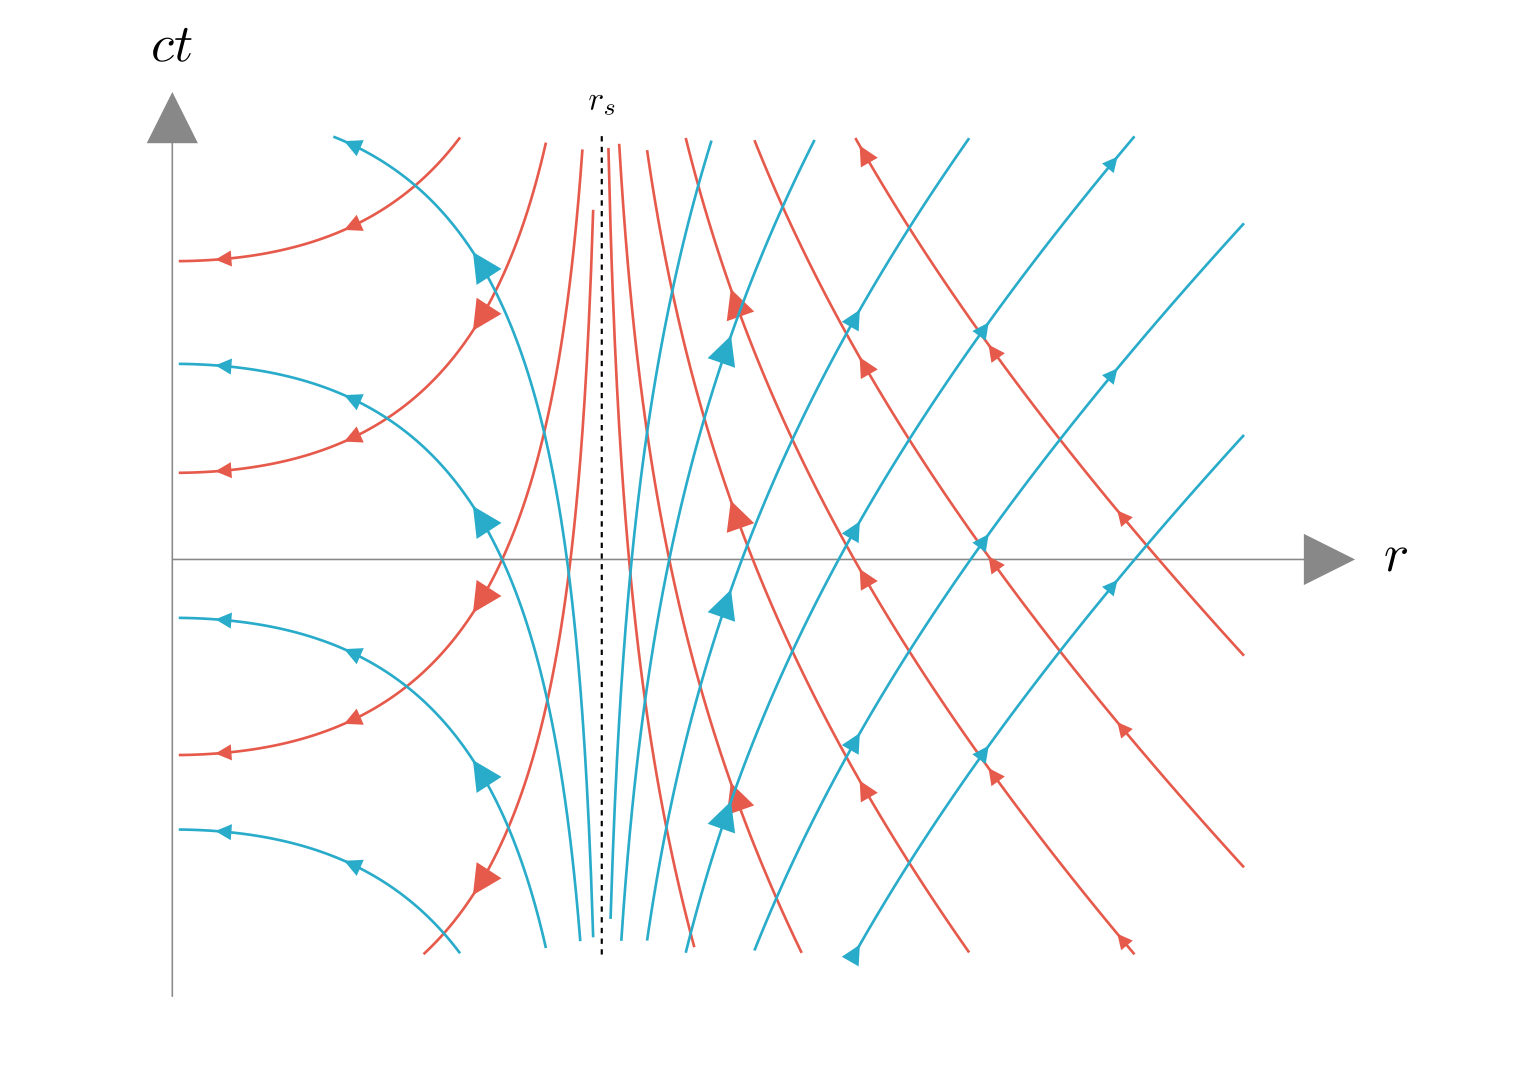
\includegraphics[width=0.95\textwidth]{AgujerosNegros/Schwarzschild/media/images/rayos_Luz_Schwarzschild_ManimCE_v0.19.0.png}
        \end{center}
        \caption{}
        \label{fig:lightraysSchwarzschild}
    \end{small}
\end{figure}

\subsection{ordenadas Eddington-Finkelstein}
Las coordenadas de Eddington-Finkelstein son un sistema de coordenadas para la solución de Schwarzschild cuya idea principal es usar las trayectorias de la luz (geodésicas nulas radiales) para definir las coordenadas temporal y radial. Esto es posible debido a la simetría radial, donde \( \theta, \varphi = \text{cte} \implies d\Omega^2 = 0 \).
Partimos de la trayectoria de la luz en términos de la coordenada radial \( r \) y el tiempo \( ct \):
\begin{equation}
    ct(r) = \pm \left( r + r_s \log \left| \frac{r}{r_s} - 1 \right| \right) + k,
\end{equation}
donde el signo \( + \) corresponde a geodésicas salientes y \( - \) a entrantes. Introducimos las nuevas variables \( c\tilde{t} \) y \( \tilde{r} \):
\begin{equation}
    \begin{aligned}
        c\tilde{t} & = ct + r_s \log \left| \frac{r}{r_s} - 1 \right|,         \\
        ct         & = c\tilde{t} - r_s \log \left| \frac{r}{r_s} - 1 \right|.
    \end{aligned}
\end{equation}
Combinando con la ecuación de las geodésicas entrantes (\( - \)):
\begin{equation}
    c\tilde{t} - r_s \log \left| \frac{r}{r_s} - 1 \right| = -r - r_s \log \left| \frac{r}{r_s} - 1 \right| + k,
\end{equation}
simplificando y renombrando la variable $\tilde{t} \to t$:
\begin{equation}
    c\tilde{t} = -r + k \to ct= -r + k .
\end{equation}
nos da las trayectorias de la luz entrantes al agujero negro.
Introducimos la coordenada \( v \):
\begin{equation}
    \begin{aligned}
        v  & = ct + r + r_s \log \left| \frac{r}{r_s} - 1 \right|, \\
        ct & = v - r - r_s \log \left| \frac{r}{r_s} - 1 \right|.
    \end{aligned}
\end{equation}
Reemplazando en la ecuación de los rayos de luz entrantes
\begin{equation}
    \begin{aligned}
        ct =v - r - r_s \log \left| \frac{r}{r_s} - 1 \right|  = - r - r_s \log \left| \frac{r}{r_s} - 1 \right| + k,
        v = k
    \end{aligned}
\end{equation}
y para los salientes
\begin{equation}
    \begin{aligned}
        ct = v - r - r_s \log \left| \frac{r}{r_s} - 1 \right|= r + r_s \log \left| \frac{r}{r_s} - 1 \right| + k, \\
        v = 2 \left(r_s \log \left| \frac{r}{r_s} - 1 \right|\right) +k
    \end{aligned}
\end{equation}
\begin{task}{Graficar}{}
    Gráfica esto.
\end{task}
Las coordenadas finales son:
\begin{equation}
    \boxed{
        v = ct + r + r_s \log \left| \frac{r}{r_s} - 1 \right|, \quad
        r_{\text{in}} = r
    }
\end{equation}

\subsubsection{Métrica de Schwarzschild en coordenadas de Eddington-Finkelstein}
La métrica se obtiene expresando los vectores base \( e_v \) y \( e_{r_{\text{in}}} \) en términos de las bases originales \( e_{ct} \) y \( e_r \). Primero, definimos \( r^* = r + r_s \log \left| \frac{r}{r_s} - 1 \right| \), con lo que:
\begin{equation}
    v = ct + r^*, \quad r_{\text{in}} = r.
\end{equation}

Las derivadas parciales para los vectores base son:
\begin{equation}
    \begin{aligned}
        e_v               & = \frac{\partial ct}{\partial v} e_{ct} + \frac{\partial r}{\partial v} e_r = e_{ct},                                                            \\
        e_{r_{\text{in}}} & = \frac{\partial ct}{\partial r_{\text{in}}} e_{ct} + \frac{\partial r}{\partial r_{\text{in}}} e_r = -\frac{1}{1 - \frac{r_s}{r}} e_{ct} + e_r.
    \end{aligned}
\end{equation}

Calculando \( \frac{dr^*}{dr} \):
\begin{equation}
    \frac{dr^*}{dr} = 1 + \frac{r_s}{r - r_s} = \frac{1}{1 - \frac{r_s}{r}}.
\end{equation}

Los componentes de la métrica \( g_{\mu\nu} = e_\mu \cdot e_\nu \) son:
\begin{equation}
    \begin{aligned}
        g_{vv}          & = e_v \cdot e_v = -\left(1 - \frac{r_s}{r}\right), \\
        g_{vr} = g_{rv} & = e_v \cdot e_{r_{\text{in}}} = 1,                 \\
        g_{rr}          & = e_{r_{\text{in}}} \cdot e_{r_{\text{in}}} = 0.
    \end{aligned}
\end{equation}
Por lo tanto, la métrica en coordenadas de Eddington-Finkelstein es:
\begin{equation}
    ds^2 = -\left(1 - \frac{r_s}{r}\right) dv^2 + 2 dv dr + r^2 d\Omega^2.
\end{equation}
\subsubsection{Coordenadas salientes de Eddington-Finkelstein}
Para geodésicas nulas salientes (\(+\)), partimos de:
\begin{equation}
    ct(r) = r + r_s \log \left| \frac{r}{r_s} - 1 \right| + k.
\end{equation}
Introducimos la coordenada \( u \):
\begin{equation}
    \begin{aligned}
        u  & = ct - r - r_s \log \left| \frac{r}{r_s} - 1 \right|, \\
        ct & = u + r + r_s \log \left| \frac{r}{r_s} - 1 \right|.
    \end{aligned}
\end{equation}
Para rayos salientes (\(+\)):
\begin{equation}
    \begin{aligned}
        u + r + r_s \log \left| \frac{r}{r_s} - 1 \right| = r + r_s \log \left| \frac{r}{r_s} - 1 \right| + k, \\
        u = k.
    \end{aligned}
\end{equation}
Y para los entrantes (\(-\)):
\begin{equation}
    \begin{aligned}
        u + r + r_s \log \left| \frac{r}{r_s} - 1 \right| = -r - r_s \log \left| \frac{r}{r_s} - 1 \right| + k, \\
        u = -2\left(r + r_s \log \left| \frac{r}{r_s} - 1 \right|  \right) +k.
    \end{aligned}
\end{equation}
\begin{task}{Graficar}{}
    Gráfica esto.
\end{task}
Las coordenadas finales son:
\begin{equation}
    \boxed{u = ct - r - r_s \log \left| \frac{r}{r_s} - 1 \right|, \quad r_{\text{out}} = r}.
\end{equation}

\subsubsection{Métrica en coordenadas salientes}

Definiendo \( r^* = r + r_s \log \left| \frac{r}{r_s} - 1 \right| \), tenemos:
\begin{equation}
    u = ct - r^*, \quad r_{\text{out}} = r.
\end{equation}

Vectores base en términos de \( e_{ct} \) y \( e_r \):
\begin{equation}
    \begin{aligned}
        e_u                & = \frac{\partial ct}{\partial u} e_{ct} + \frac{\partial r}{\partial u} e_r = e_{ct},                                                             \\
        e_{r_{\text{out}}} & = \frac{\partial ct}{\partial r_{\text{out}}} e_{ct} + \frac{\partial r}{\partial r_{\text{out}}} e_r = \frac{1}{1 - \frac{r_s}{r}} e_{ct} + e_r.
    \end{aligned}
\end{equation}

Componentes de la métrica \( g_{\mu\nu} = e_\mu \cdot e_\nu \):
\begin{equation}
    \begin{aligned}
        g_{uu}          & = e_u \cdot e_u = -\left(1 - \frac{r_s}{r}\right), \\
        g_{ur} = g_{ru} & = e_u \cdot e_{r_{\text{out}}} = -1,               \\
        g_{rr}          & = e_{r_{\text{out}}} \cdot e_{r_{\text{out}}} = 0.
    \end{aligned}
\end{equation}

La métrica en coordenadas salientes es:
\begin{equation}
    ds^2 = -\left(1 - \frac{r_s}{r}\right) du^2 - 2 du dr + r^2 d\Omega^2.
\end{equation}


En estas coordenadas:
\begin{itemize}
    \item Líneas con \( u = \text{cte} \) son geodésicas salientes con pendiente \( +1 \) en diagramas espacio-temporales.
    \item La métrica es regular en \( r = r_s \), eliminando la singularidad coordenada de Schwarzschild.
    \item \( r_{\text{out}} \) coincide con la coordenada radial areal.
\end{itemize}
\begin{itemize}
    \item Mostrar que las partículas de luz/masivas pueden pasar a través del horizonte de eventos, pero...
    \item En coordenadas de EF entrantes: los haces de luz salientes no funcionan en $r_s$
    \item En coordenadas de EF salientes: los haces de luz entrantes no funcionan en $r_s$
\end{itemize}


\subsection{Coordenadas Kruskal-Szekeres}

\subsubsection{Coordenadas nulas originales}
Definimos las coordenadas entrante (\(v\)) y saliente (\(u\)) de Eddington-Finkelstein:
\begin{equation}
    \begin{aligned}
        v   & = ct + r^*                                      \\
        u   & = ct - r^*                                      \\
        r^* & \equiv r + r_s \log\left|\frac{r}{r_s}-1\right|
    \end{aligned}
\end{equation}

\subsubsection{Vectores base en coordenadas \( (u, v) \)}
Expresamos los vectores base en términos de \( e_{ct} \) y \( e_r \):
\begin{equation}
    \begin{aligned}
        e_v & = \frac{\partial ct}{\partial v}e_{ct} + \frac{\partial r}{\partial v}e_r = \frac{1}{2}e_{ct} + \frac{1}{2}\left(1-\frac{r_s}{r}\right)^{-1}e_r \\
        e_u & = \frac{\partial ct}{\partial u}e_{ct} + \frac{\partial r}{\partial u}e_r = \frac{1}{2}e_{ct} - \frac{1}{2}\left(1-\frac{r_s}{r}\right)^{-1}e_r
    \end{aligned}
\end{equation}

\subsubsection{Productos punto fundamentales}
Usando la métrica de Schwarzschild \( g(e_{ct},e_{ct}) = -\left(1-\frac{r_s}{r}\right) \) y \( g(e_r,e_r) = \left(1-\frac{r_s}{r}\right)^{-1} \):
\begin{equation}
    \begin{aligned}
        e_v \cdot e_v & = \left(\frac{1}{2}\right)^2 g(e_{ct},e_{ct}) + \left(\frac{1}{2}\left(1-\frac{r_s}{r}\right)^{-1}\right)^2 g(e_r,e_r) = 0                                        \\
        e_u \cdot e_u & = \left(\frac{1}{2}\right)^2 g(e_{ct},e_{ct}) + \left(\frac{1}{2}\left(1-\frac{r_s}{r}\right)^{-1}\right)^2 g(e_r,e_r) = 0                                        \\
        e_v \cdot e_u & = \left(\frac{1}{2}\right)^2 g(e_{ct},e_{ct}) - \left(\frac{1}{2}\left(1-\frac{r_s}{r}\right)^{-1}\right)^2 g(e_r,e_r) = -\frac{1}{2}\left(1-\frac{r_s}{r}\right)
    \end{aligned}
\end{equation}

\subsubsection{Métrica en coordenadas nulas}
La métrica se expresa como:
\begin{equation}
    ds^2 = 2(e_v \cdot e_u) du\, dv + r^2 d\Omega^2 = -\left(1-\frac{r_s}{r}\right) du\, dv + r^2(d\theta^2 + \sin^2\theta d\varphi^2)
\end{equation}

\subsubsection{Transformación a Kruskal-Szekeres}

\begin{equation}
    \begin{aligned}
        \frac{v-u}{2}=r+r_s \log \left|\frac{r}{r_s}-1\right|                 \\
        \frac{v-u}{2 r_s}=\frac{r}{r_s}+\log \left|\frac{r}{r_s}-1\right|     \\
        e^{\frac{v-u}{2 r_s}}=e^{\frac{r}{r_s}+\log \abs{ \frac{r}{r_s} 1} }, \\
        -e^{\frac{v}{2 r_s}}\left(-e^{-\frac{u}{2 r_s}}\right)=e^{\frac{r}{r_s}}\left|\frac{r}{r_s}-1\right|
    \end{aligned}
\end{equation}
Definimos las nuevas coordenadas:
\begin{equation}
    \mathcal{U} = -e^{-\frac{u}{4r_s}}, \quad \mathcal{V} = e^{\frac{v}{4r_s}}
\end{equation}

\subsubsection{Vectores base en Kruskal-Szekeres}
Relación diferencial usando la regla de la cadena:
\begin{equation}
    \begin{aligned}
        e_\mathcal{U} & = \frac{\partial u}{\partial \mathcal{U}} e_u = 4r_s e^{\frac{u}{4r_s}} e_u = -4r_s \mathcal{U}^{-1} e_u \\
        e_\mathcal{V} & = \frac{\partial v}{\partial \mathcal{V}} e_v = 4r_s e^{-\frac{v}{4r_s}} e_v = 4r_s \mathcal{V}^{-1} e_v
    \end{aligned}
\end{equation}

\subsubsection{Producto punto clave}
Calculamos el producto punto usando \( e_u \cdot e_v = -\frac{1}{2}\left(1-\frac{r_s}{r}\right) \):
\begin{equation}
    e_\mathcal{U} \cdot e_\mathcal{V} = (-4r_s \mathcal{U}^{-1})(4r_s \mathcal{V}^{-1})(e_u \cdot e_v) = \frac{8r_s^2}{\mathcal{U}\mathcal{V}}\left(1-\frac{r_s}{r}\right)
\end{equation}

\subsubsection{Relación geométrica fundamental}
De la definición de \( \mathcal{U} \) y \( \mathcal{V} \):
\begin{equation}
    \mathcal{U}\mathcal{V} = -e^{\frac{r^*}{2r_s}} = -\left|\frac{r}{r_s}-1\right|^{1/2}e^{\frac{r}{2r_s}}
\end{equation}

Sustituyendo en el producto punto:
\begin{equation}
    e_\mathcal{U} \cdot e_\mathcal{V} = \frac{32r_s^3}{r}e^{-\frac{r}{r_s}}
\end{equation}

\subsubsection{Métrica final de Kruskal-Szekeres}
La métrica toma su forma canónica:
\begin{equation}
    \boxed{ds^2 = \frac{32r_s^3}{r}e^{-\frac{r}{r_s}} d\mathcal{U}d\mathcal{V} + r^2(d\theta^2 + \sin^2\theta d\varphi^2)}
\end{equation}

\begin{equation}
    \text{con } \mathcal{U}\mathcal{V} = \left(1-\frac{r}{r_s}\right)e^{\frac{r}{r_s}} \quad \text{y} \quad \frac{\mathcal{V}}{\mathcal{U}} = -e^{\frac{ct}{2r_s}}
\end{equation}
De momento $\mathcal{V}$ y $\mathcal{U}$ son coordenadas nulas, que describen trayectorias de luz, pero podemos hacerlas espaciales y temporales definiendo:
\begin{equation}
    \begin{aligned}
        T \equiv \frac{\mathcal{V}+\mathcal{U}}{2} \\
        X \equiv \frac{\mathcal{V}-\mathcal{U}}{2} \\
    \end{aligned}
\end{equation}
y viceversa
\begin{equation}
    \begin{aligned}
        \mathcal{V}=T+X \\
        \mathcal{U}=T-X
    \end{aligned}
\end{equation}
De modo que la métrica en términos de $T$ y $X$ es:
\begin{equation}
        g_{\mu \nu} =\left[\begin{array}{cccc}
                                             +\frac{4 r_s^3}{r} e^{-\frac{r}{r_s}} & 0                                     & 0    & 0                   \\
                                             0                                     & -\frac{4 r_s^3}{r} e^{-\frac{r}{r_s}} & 0    & 0                   \\
                                             0                                     & 0                                     & -r^2 & 0                   \\
                                             0                                     & 0                                     & 0    & -r^2(\sin \theta)^2
                                         \end{array}\right]
\end{equation}
Usando el mismo truco que usamos anteriormente podemos encontar las geodésicas nulas en estas coordenadas.
\begin{equation}
    \begin{array}{l}
        0=\left(\frac{d T}{d \lambda}\right)^2\left(\frac{\partial}{\partial T} \cdot \frac{\partial}{\partial T}\right)+\left(\frac{d X}{d \lambda}\right)^2\left(\frac{\partial}{\partial X} \cdot \frac{\partial}{\partial X}\right) \\
        0=\left(\frac{d T}{d \lambda}\right)^2 g_{T T}+\left(\frac{d X}{d \lambda}\right)^2 g_{X X}                                                                                                                                     \\
        0=\left(\frac{d T}{d \lambda}\right)^2\left(+2 g_{U V}\right)+\left(\frac{d X}{d \lambda}\right)^2\left(-2 g_{U V}\right)
    \end{array}
\end{equation}

\begin{equation}
    \d{X}{\lambda} =\pm \d{T}{\lambda} \to \d{X}{T} = \pm 1 \to T = \pm Y + k
\end{equation}

Eso quiere decir que las geodésicas nulas en estas coordenadas son rectas en el espacio-tiempo. 
ahora volver a poner las coordenadas en términos de $r$ y $t$ solo es cuestión de una composición de funciones.

\begin{equation}
    \begin{aligned}
        T&=\frac{V+U}{2} \\
        X&=\frac{V-U}{2}
    \end{aligned}
    \quad ; 
    \begin{aligned}
        V&=e^{\frac{v}{2 r_s}} \\
        U&=-e^{-\frac{u}{2 r_s}}
    \end{aligned}
    \quad ; 
    \begin{aligned}
        v&=c t+r+r_s \log \left|\frac{r}{r_s}-1\right| \\
        u&=c t-r-r_s \log \left|\frac{r}{r_s}-1\right|
    \end{aligned}
\end{equation}
Simplificando
\begin{equation}
    \begin{aligned}
        T & =  \frac{1}{2}\left(V + U\right)                                                                                                                                                      \\
          & = \frac{1}{2} e^{\frac{v}{2 r_s}}-\frac{1}{2} e^{-\frac{u}{2 r_S}}                                                                                                                    \\
          & = \frac{1}{2} e^{\frac{1}{2 r_s}\left(c t+r+r_s \log \left|\frac{r}{r_s}-1\right|\right)}-\frac{1}{2} e^{-\frac{1}{2 r_s}\left(c t-r-r_s \log \left|\frac{r}{r_s}-1\right|\right)}    \\
          & =\frac{1}{2} e^{\frac{c t}{2 r_s}} e^{\frac{r}{2 r_s}}\left(\left|\frac{r}{r_s}-1\right|\right)^{1 / 2}-\frac{1}{2} e^{\frac{-c t}{2 r_s}} e^{\frac{r}{2 r_s}}\left(\left|\frac{r}{r_s}-1\right|\right)^{1 / 2} \\
          & = e^{\frac{r}{2 r_s}} \sqrt{\left|\frac{r}{r_s}-1\right|} \frac{1}{2}\left(e^{\frac{c t}{2 r_s}}-e^{\frac{-c t}{2 r_s}}\right)                                                                     \\
          & = e^{\frac{r}{2 r_s}} \sqrt{\left|\frac{r}{r_s}-1\right|} \sinh\left(\frac{ct}{2r_s}\right)
          \label{eq:Kruskal-SzekeresT(r,t)}
    \end{aligned}
\end{equation}
y para $X$ el calculo es prácticamente el mismo a excepción de un signo ($+$) en la diferencia de exponentes.
\begin{equation}
        X  = e^{\frac{r}{2 r_s}} \sqrt{\left|\frac{r}{r_s}-1\right|}  \cosh\left(\frac{ct}{2r_s}\right)
        \label{eq:Kruskal-SzekeresX(r,t)}
\end{equation}
Donde podemos desarrollar la siguiente identidad
\begin{equation}
    \begin{aligned}
        T^2 - X^2 &= \left( e^{\frac{r}{2r_s}} \sqrt{\left|\frac{r}{r_s}-1\right|}\, \sinh\left(\frac{ct}{2r_s}\right) \right)^2 
        - \left( e^{\frac{r}{2r_s}} \sqrt{\left|\frac{r}{r_s}-1\right|}\, \cosh\left(\frac{ct}{2r_s}\right) \right)^2\\[1mm]
        &= e^{\frac{r}{r_s}} \left|\frac{r}{r_s}-1\right| \left[ \sinh^2\left(\frac{ct}{2r_s}\right) - \cosh^2\left(\frac{ct}{2r_s}\right) \right]\\[1mm]
        &= -\, e^{\frac{r}{r_s}} \left|\frac{r}{r_s}-1\right|\\[2mm]
        &=
        \begin{cases}
            -\, e^{\frac{r}{r_s}} \left(\dfrac{r}{r_s}-1\right), & \text{si } r > r_s,\\[2mm]
            -\, e^{\frac{r}{r_s}} \left(1-\dfrac{r}{r_s}\right), & \text{si } r < r_s.
        \end{cases}
    \end{aligned}
    \label{eq:Kruskal-SzekeresT^2-X^2}
\end{equation}
\begin{task}{Demostrar}{}
    Demostrar la identidad (\ref{eq:Kruskal-SzekeresT^2-X^2}).
\end{task}
Esta identidad nos ayuda a determinar las líneas de \(r\) constante en el espacio-tiempo de Schwarzschild. Lo interesante ocurre cuando observamos el caso \(r < r_s\): el valor absoluto \(\left|\frac{r}{r_s}-1\right|\) en la ecuación (\ref{eq:Kruskal-SzekeresT^2-X^2}) se puede expresar como \(1-\frac{r}{r_s}\). ¿Por qué es importante notar esto? Si nos fijamos en la segunda línea de la ecuación, podemos identificar los coeficientes de la siguiente forma:
\begin{equation}
    \begin{aligned}
        T^2 - X^2 &= e^{\frac{r}{r_s}} \left(1-\frac{r}{r_s}\right) \left[ \sinh^2\left(\frac{ct}{2r_s}\right) - \cosh^2\left(\frac{ct}{2r_s}\right) \right] \\
        &= -\, e^{\frac{r}{r_s}} \left(\frac{r}{r_s}-1\right) \left[ \sinh^2\left(\frac{ct}{2r_s}\right) - \cosh^2\left(\frac{ct}{2r_s}\right) \right] \\
        &= e^{\frac{r}{r_s}} \left(\frac{r}{r_s}-1\right) \left[ \cosh^2\left(\frac{ct}{2r_s}\right) - \sinh^2\left(\frac{ct}{2r_s}\right) \right].
    \end{aligned}
\end{equation}
De ello se deduce que, dentro del horizonte de eventos (\(r < r_s\)), se tienen las siguientes expresiones:
\begin{equation}
    X = e^{\frac{r}{2r_s}} \sqrt{1-\frac{r}{r_s}} \, \frac{1}{2} \sinh\left(\frac{ct}{2r_s}\right), \quad 
    T = e^{\frac{r}{2r_s}} \sqrt{1-\frac{r}{r_s}} \, \frac{1}{2} \cosh\left(\frac{ct}{2r_s}\right).
\end{equation}
Dado que el negativo de estas coordenadas $-X$ y $-T$ cumplen la identidad (\ref{eq:Kruskal-SzekeresT^2-X^2}) podemos escribir lo que se llama la extensión máxima de las coordenadas de Kruskal-Szekeres
\begin{table}[H]
    \centering
    \caption{Extensión máxima de las coordenadas de Kruskal-Szekeres}
    \begin{tabular}{|c|c|c|}
        \hline Region & $T$                                                                                         & $X$                                                                                \\
        \hline$I$        & $+\sinh \left(\frac{c t}{2 r_s}\right)\frac{r}{2 r_s} \sqrt{\frac{r}{r_s}-1}$ & $+\cosh \left(\frac{c t}{2 r_s}\right) e^{\frac{r}{2 r_s}} \sqrt{\frac{r}{r_s}-1}$ \\
        \hline$I I$       & $+\cosh \left(\frac{c t}{2 r_s}\right) e^{\frac{r}{2 r_s}} \sqrt{1-\frac{r}{r_s}}$          & $+\sinh \left(\frac{c t}{2 r_s}\right) e^{\frac{r}{2 r_s}} \sqrt{1-\frac{r}{r_s}}$ \\
        \hline$I I I$   & $-\sinh \left(\frac{c t}{2 r_s}\right) e^{\frac{r}{2 r_s}} \sqrt{\frac{r}{r_s}-1}$          & $-\cosh \left(\frac{c t}{2 r_s}\right) e^{\frac{r}{2 r_s}} \sqrt{\frac{r}{r_s}-1}$ \\
        \hline$I V$      & $-\cosh \left(\frac{c t}{2 r_s}\right) e^{\frac{r}{2 r_s}} \sqrt{1-\frac{r}{r_s}}$          & $-\sinh \left(\frac{c t}{2 r_s}\right) e^{\frac{r}{2 r_s}} \sqrt{1-\frac{r}{r_s}}$ \\
        \hline
    \end{tabular}
\end{table}
Ahora para la lineas de tiempo constante es fácil ver la siguiente relación
\begin{equation}
    \tanh \left(\frac{ct}{2 r_s}\right)=\left\{\begin{array}{ll}
        T / X & \text { (en region I y III) } \\
        X / T & \text { (en region II y IV) }
        \end{array}\right.
\end{equation}
Con esto tenemos todo lo necesario para construir el diagrama de Kruskal-Szekeres.  
\begin{figure}[H]
    \begin{small}
        \begin{center}
            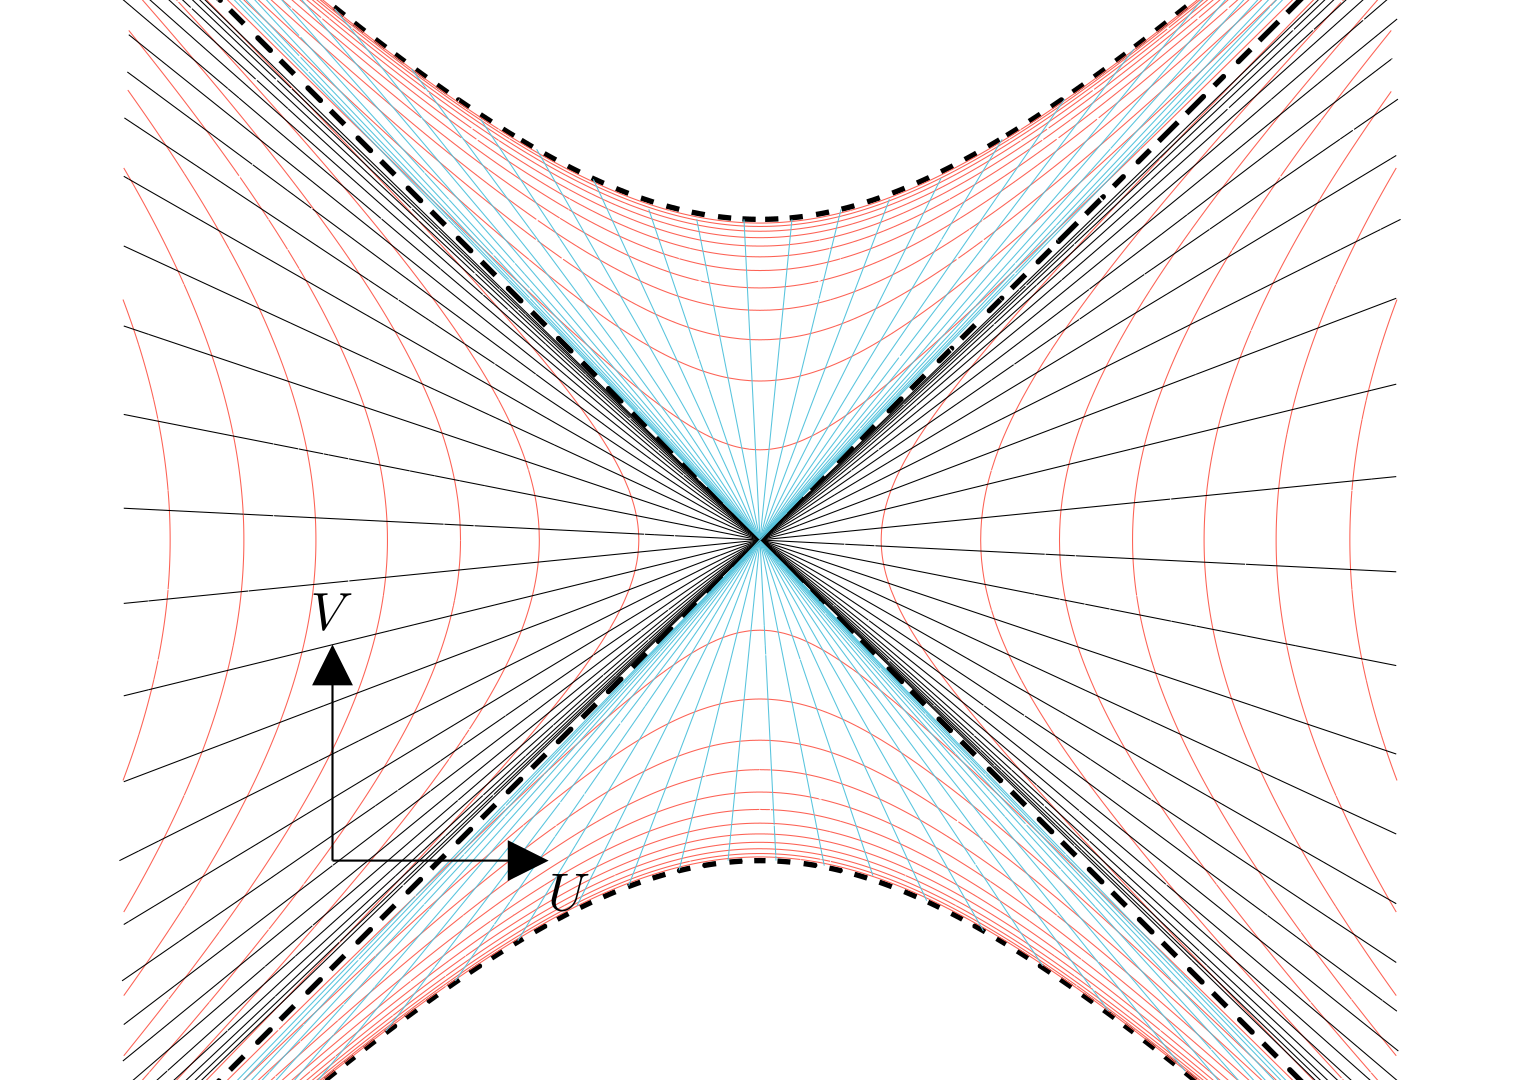
\includegraphics[width=0.95\textwidth]{AgujerosNegros/Schwarzschild/media/images/Kruskal_Szekeres_diagram_ManimCE_v0.19.0.png}
        \end{center}
        \caption{}
        \label{fig:}
    \end{small}
\end{figure}
